\chapter[Achievable Rates]{Mean Achievable Rates in Clustered Coordinated Base
Station Transmission with Block Diagonalization\footnote{
    The work shown in this chapter has been published in \cite{corvaja13b}.
}} \label{ch:achiev_rates}

%-------------------------------------------------------------------------------
\section{Introduction}\label{sec:achiev_introduction}

In \verb+\refc{ch:state_art}+ it has been discussed how global coordination in a
cellular network is not feasible for practical application. Research has shown
that grouping cells in clusters may help to alleviate some of the problems of
global coordination. The clustering solution is not unique, though, and multiple
alternatives an numerous parameters have to be chosen in order to meet different
objectives.

The objective of this chapter is to analyze the mean achievable rate in a cellular network where clusters have been formed, and where \gls{bd} is used within
each cluster to manage the interference. 

With this analysis, further research can be made in order to be able to choose
from one of the most important parameters in clustering, the cluster size.

Numerical simulations are also performed in order to validate the theoretical
analysis developed.

%-------------------------------------------------------------------------------
\section{Clustered Network}\label{sec:achiev_clust_net}

The network to be considered is organized as independent groups of $M$ cells,
each of which is a cluster where its cells coordinate in order to transmit to
the $N$ users that are located within the cluster.

The clusters that form the network are non-overlapping, \emph{i.e.} each cell in
the system belongs to one and only one cluster. Overlapping, user-centric
clusters have been shown to provide, in some situations, better performance than
disjoint clusters \cite{bjornson11}, but this approach gives rise to a dramatic
increase of the management complexity.

The clusters, then, are defined by the network planner, and they are kept fixed,
grouping the \gls{bs} according to a distance criterion, so that the cells
belonging to a cluster must form, borrowing the name from graph theory, a
\emph{connected component} of the graph containing all the cells in the system.

In the setup under study, all the \gls{bs} in the cluster are considered cluster
members, that is, no scheduling or adaptive selection of active \gls{bs} is
addressed in this work. In any case, they could be considered as a special case
of the optimization problem to obtain the power allocation scheme.

\begin{figure}[t]
\begin{center}
    \dummybox
% \hspace*{1mm}\input ./Fig2.tex
\end{center}
\caption{System layout with clusters of seven cells of radius $\Rcell$ (the
radius of the circle circumscribing the cell) with an example of two users,
with the distances $\Dtone$ and $\Dttwo$, respectively, from their \gls{bs} to
the interfering \gls{bs}.}
\label{fig:achiev_cluster_layout}
\end{figure}

\reff{fig:achiev_cluster_layout} shows such a clustered network, where the
disjoint clusters can be observed, together with other parameters that will be
used in considering the interference for the analysis.

%-------------------------------------------------------------------------------
\section{Interference Model}\label{sec:achiev_interf}

In \reff{fig:achiev_cluster_layout} an example of a network is shown, with three
complete clusters of $M=7$ cells each, and with some cells belonging to clusters
not completely shown.

The user $i$, at a distance $d_i$ from its serving \gls{bs}, \emph{cf.}
\refs{sec:system_model}, is affected by the interference originated in the
neighboring clusters. In this case, the closest interfering cells are located at
a distance $\Dtone = \sqrt{3} \Rcell$ from the $i$-th \gls{bs}.

Similarly, for the user $j$, at a distance $d_j$ from its serving \gls{bs},
\emph{cf.} \refs{sec:system_model}, the nearest interfering cells are located at
a distance $\Dttwo = 3\Rcell$ from the $j$-th \gls{bs}.

Due to the cellular geometry, for a cluster size of up to 18, only these two
possibilities exist: the closest interfering cell is at a distance of either
$\Dtone$ or $\Dttwo$ from the serving \gls{bs} of each user.

The hexagonal cell can be approximated by a circular one with radius $\Rcell$,
see \reff{fig:achiev_cluster_layout}, and then, assuming a uniform distribution
of the users over each cell, the \gls{pdf} of the distance of a user to its
serving (closest) \gls{bs} is given by

\begin{equation} \label{eq:pdf_distance}
    f_{d_i}\left(d_i\right) = \frac{2d_i}{\Rcell^2}
\end{equation}

The interference power received at the user $i$ is equal to

\begin{equation} \label{eq:interf_power}
    I_i\left( d_i \right) = \sum\limits_{m=1}^{\Minterf}P_{\max}
    \hat{d}_{im}^{-\gamma}
\end{equation}

\noindent
where $\Minterf$ is the number of interfering \gls{bs}, \emph{i.e.} the total
number of cells in the system minus the $M$ cells that form the cluster, and
$\hat{d}_{im}$ is the distance from the $m$-th \gls{bs} outside the cluster to
the $i$-th user in the cluster. All the interfering \gls{bs} are assumed to be
transmitting at full power.

In order to simplify the computation of the interference power, an equivalent
model is introduced. In this model, the interference comes from $\Meqi$ cells,
all of which are located at the same distance $\left(D_i - d_i\right)$ from the
$i$-th user, the one being interfered. 

The distance $D_i$ takes the value of the distance from the serving \gls{bs} to
the closest interfering \gls{bs}

\begin{equation} \label{eq:interf_min_dist}
    D_i \in \left\{ \Dtone, \Dttwo \right\}
\end{equation}

The equivalent number of interfering \gls{bs}, $\Meqi$, is such that the total
interference power is the same as in the original layout.

With all this, \eqref{eq:interf_power} can be written as

\begin{equation} \label{eq:interf_power_eq}
    I_i\left(d_i\right) = P_{\max}\Meqi\left(D_i - d_i\right)^{-\gamma}
\end{equation}

This approach is similar to that followed in \cite{cheikh11}, where a fluid
model network is used. This model assumes that there is a continuum of \gls{bs}
interfering, but this will not be considered in the current work for the sake of
simplicity.

The real and equivalent model produce the same total interference, provided that
$\Meqi$ is adequately selected.

In order to determine $\Meqi$ the only interference that is accounted for is the
one coming from the first tier of neighboring cells. This implies that different
cluster configurations may have different number of interfering \gls{bs} for
each of the cells in the cluster, and this number for the $i$-th cell is denoted
as $\Minti \leq \Minterf$.

\begin{figure}[t]
\begin{center}
    \dummybox
% \hspace*{-8mm}\input ./Fig3.tex
\end{center}
\caption{Cluster with $M=4$ cells and neighbor interfering cells.}
\label{fig:cluster_interf_cells}
\end{figure}

This is made clear in \reff{fig:cluster_interf_cells} where a cluster with
$M = 4$ cells is surrounded by $\Minterf = 12$ cells. In this cluster, cells 1
and 3 experience an interference coming from $M_{\text{int}, 1} =
M_{\text{int}, 3} = 4$ neighboring cells, while cells 2 and 4 receive the
interference from $M_{\text{int}, 2} = M_{\text{int}, 4} = 3$ cells.

In order to approximate the value of equivalent interfering \gls{bs} for a
general network setup, fist consider a simple scenario \reff{fig:cluster_1} with
a cluster of $M = 1$ cells, where a single user, $i = 1$, in the cell is
affected by an interference power $I_1$ coming from all the
$M_{\text{int}, 1} = 6$ belonging to the first tier.

\begin{figure}[t]
\begin{center}
    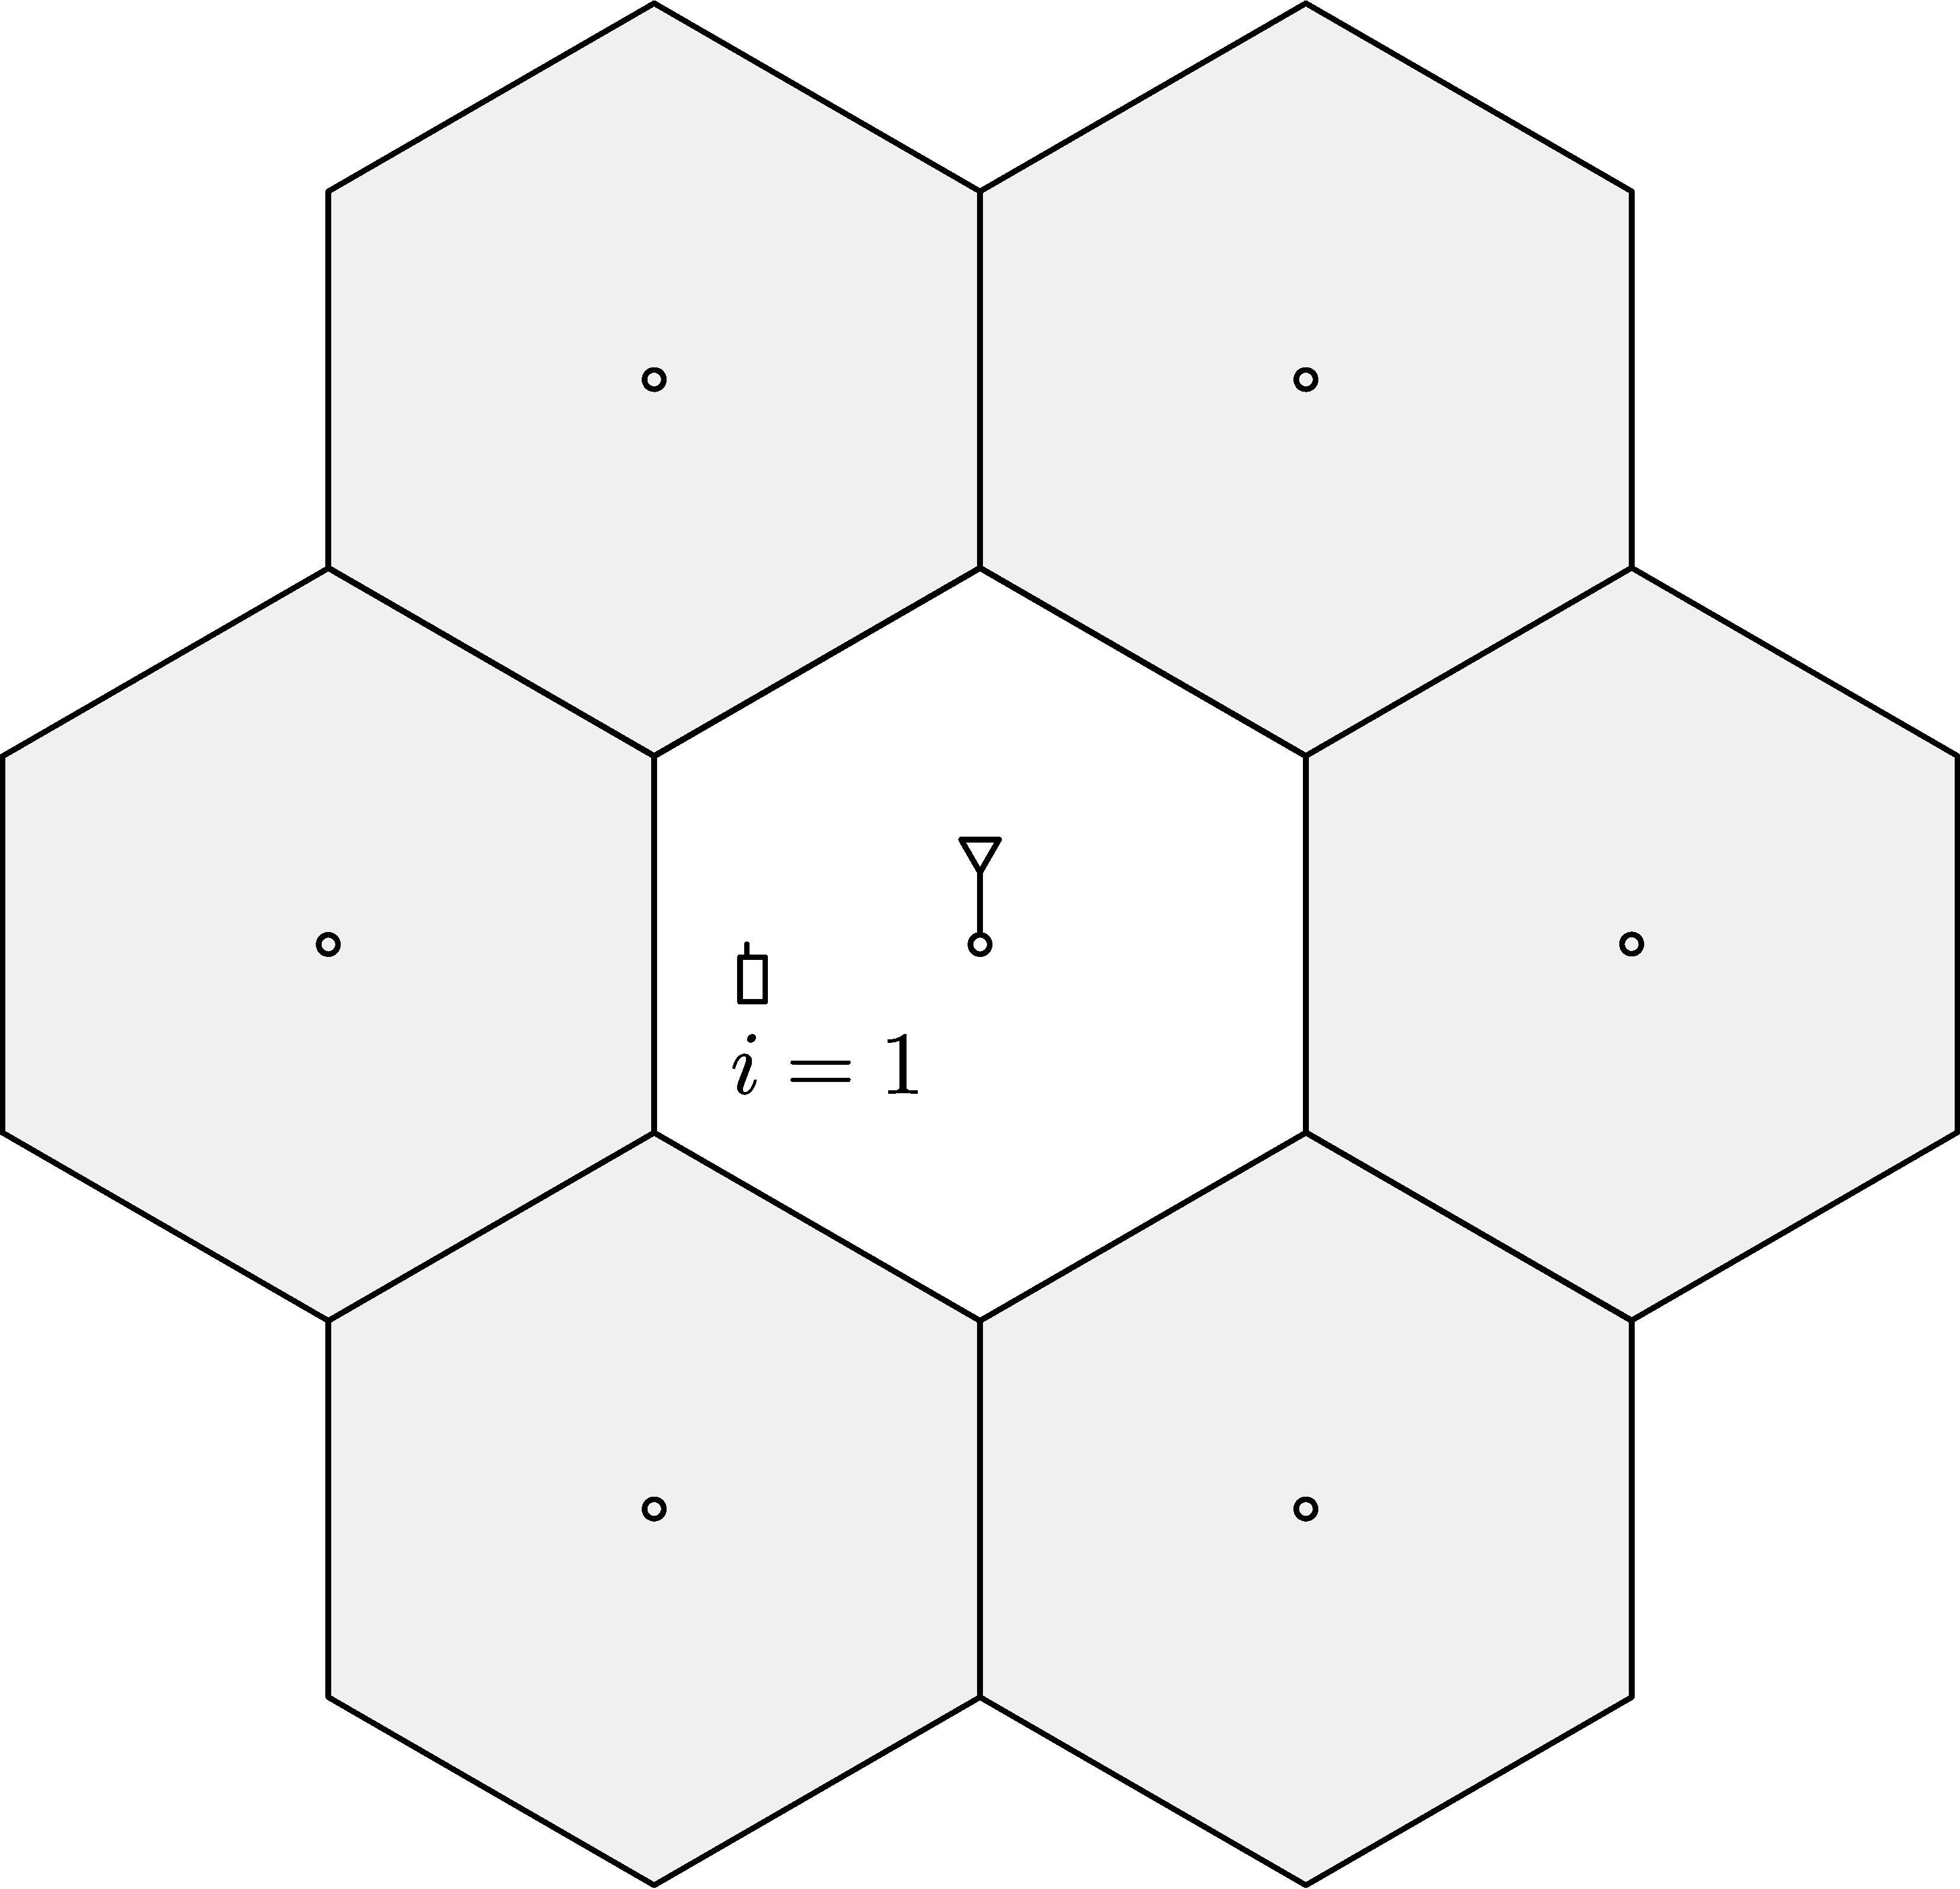
\includegraphics[width=0.8\textwidth]{./10.achievable_rates/img/cluster_1}
\end{center}
\caption{Simple scenario with a single cluster of $M = 1$ cell, and the six
    interfering cells surrounding it.}
\label{fig:cluster_1}
\end{figure}

An assumption that can be made is that half of the $M_{\text{int}, 1}$, \emph{i.e.} three, \gls{bs} are located at a distance $\left( D_1 - d_1 \right)$ and the
other half are located at a distance $\left( D_1 + d_1 \right)$. Accordingly,
the interference power can be expressed as

\begin{equation} \label{eq:interf_cluster_1}
    I_1\left(d_1\right) = P_{\max} \left[ \frac{3}{\left(D_1 + d_1
        \right)^\gamma} + \frac{3}{\left(D_1 + d_1 \right)^\gamma}\right]
\end{equation}

\noindent
which is equal to \eqref{eq:interf_power_eq} if the equivalent number of
interfering \gls{bs} is defined as

\begin{equation} \label{eq:meq_cluster_1}
    M_{\text{eq},1} = 3 \left[ 1 + \left(\frac{D_1 - d_1}{D_1 + d_1}
    \right)^\gamma\right]
\end{equation}

In general, if a user $i$ is considered to have $M_{\text{int}, i}$ interfering
\gls{bs} in the first tier at a distance $D_i$, defined as in
\eqref{eq:interf_min_dist}, then the equivalent number of interfering \gls{bs}
is given by

\begin{equation} \label{eq:general_meq}
    M_{\text{eq}, i} \approx \frac{M_{\text{int}, i}}{2} \left[ 1 + \left(
    \frac{D_i - d_i}{D_i + d_i}\right)^\gamma\right]
\end{equation}

In order to evaluate \eqref{eq:general_meq}, it is possible to set the distance
$d_i$ to the average distance of the user within the cell. A similar approach is
used in \cite{pijcke11} to characterize the statistics of the interference in a
multi-cell scenario. This average distance can be obtained from the uniform
spatial distribution in \eqref{eq:pdf_distance} as

\begin{equation} \label{eq:average_distance}
    \mathbb{E}\left\{d_i\right\} = \frac{2}{3}\Rcell
\end{equation}

\noindent
and then

\begin{equation} \label{eq:meq_cluster_generic}
    M_{\text{eq}, i} \approx \frac{M_{\text{int},i}}{2} \left[ 1 + \left(
        \frac{D_i - \frac{2}{3}\Rcell}
        {D_i + \frac{2}{3}\Rcell}\right)^\gamma\right]
\end{equation}

\refs{sec:achiev_numerical} deals with the comparison between simulations and
the analytical results, showing that the approximation in
\eqref{eq:meq_cluster_generic} is accurate.


%-------------------------------------------------------------------------------
\section{Analysis of the Rate}\label{sec:achiev_rate_analysis}

In the case of having global coordination or, equivalently, having only one
cluster including all the \gls{bs}, the interference among the users is
completely eliminated through the use of \gls{bd}, \emph{cf.} \refs{sec:bd}. On
the other hand, in a multicluster environment, it is necessary to consider the
effect of the interference coming from the cells outside the cluster. Hence, the
mean achievable rate in \eqref{eq:bd_ergodic_capacity} becomes (dropping the
expectation notation)

\begin{equation} \label{eq:rate_bd_interf}
    R_i^{\text{BD}} = \sum\limits_{k = 1}^{\ell} \log_2 \left(1 +
        \frac{\lambdahat_{ik} p_{ik}}{\sigma_i^2 + I_i} \right)
\end{equation}

\noindent
where the parameter $I_i$ represents the average power of the total interference
contributions received in each data stream of user $i$ from the interfering
\gls{bs}.

It can be seen in \eqref{eq:rate_bd_interf} that the rate depends on the distance $d_i$ of each user's equipment from the center of its cell. Using the pdf in
\eqref{eq:pdf_distance} the average of the rate over all possible locations,
making explicit the dependence on the distance $d_i$, can be expressed as

\begin{equation} \label{eq:rate_bd_loc_aver}
\begin{aligned}
    \bar{R}_i^{\text{BD}} &= \int\limits_0^{\Rcell} R_i^{\text{BD}}\left(u
    \right) \frac{2u}{\Rcell^2} \dee u \\
    &= \int\limits_0^{\Rcell} \sum\limits_{k = 1}^{\ell} \log_2 \left(1 +
    \frac{\lambdahat_{ik}\left(u\right) p_{ik}}{\sigma_i^2 + I_i\left(u\right)}
    \right) \frac{2u}{\Rcell^2} \dee u
\end{aligned}
\end{equation}

In \eqref{eq:rate_bd_loc_aver} there are three parameters that determine the
overall average rate, namely

\begin{itemize}
    \item The interference $I_i\left(d_i\right)$ coming from outside the
        cluster.
    \item The effect of the channel fading and of the path loss, represented by
        the term $\lambdahat_{ik}\left(d_i\right)$.
    \item The power $p_{ik}$ assigned to the $k$-th data stream of user $i$.
\end{itemize}

In the following, the characterization of each of these parameters will be
approached separatedly.

%-------------------------------------------------------------------------------
\subsection{Interference}\label{ssec:achiev_rate_interf}

As described in \refs{sec:achiev_interf} the contribution of interference,
$I_i\left(d_i\right)$ on each data stream of user $i$, coming from the cells
outside the cluster, can be considered as generated by an equivalent number of
\gls{bs} located all of them at a distance of $D_i - d_i$ from the user. Recall
that, for clusters of size up to 18, $D_i$ can take one of two values as in
\eqref{eq:interf_min_dist}.

The interfering distance $D_i$ is then normalized to the cell radius $\Rcell$ by
setting

\begin{equation} \label{eq:interf_dist_norm}
    \bar{d}_i = \frac{D_i}{\Rcell}
\end{equation}

In expression \eqref{eq:rate_bd_interf} it is assumed that the interference can
be treated as Gaussian noise, so that the power is calculated as the variance
of that noise. Throughout the simulations that were performed, it has been found
that, on average, at least 25 out-of-cluster cells contributed with significant
interference.\footnote{Being significant defined as being greater than the power
received at the cell edge.}

This number of 25 is dependent on the simulation paremeters, but it gives an
idea of the order of magnitud of interferers present, and it justifies the
treatment of the interference as Gaussian noise, by virtue of the central limit
theorem \cite{papoulis_fourier}.

%-------------------------------------------------------------------------------
\subsection{Fading Effect}\label{ssec:achiev_rate_fading}

The terms $\lambdahat_{ij}$ are the squared diagonal values of the matrix
$\bLambdahat_i$, \emph{cf.} \refs{sec:bd}. This matrix is obtained in
\eqref{eq:svd_max_rate} by the combination of the channel matrix $\HH_i$ and a
unitary matrix, $\Vtilde_i^{(0)}$.

The channel matrix $\HH_i$ is composed of the submatrices $\HH_{ij}$, where the
fading elements have a power path loss of $d_{ij}^{-\gamma}$, and the elements
of $\HH_{ij}$ are independent from the elements of $\HH_{ik}$ for all $j$
different from $k$.

It is possible to define an alternative set of coefficients $\kappa_{ij}$ that
do not include the path loss effect

\begin{equation} \label{eq:kappa_coeff}
    \kappa_{ij} \triangleq \frac{\lambdahat_{ij}}{d_{i}^{-\gamma}}
\end{equation}

These coefficientes are the elements of the main diagonal of the matrix

\begin{equation} \label{eq:diag_matrix_no_path_loss}
    d_{i}^{\gamma}\bLambdahat_i \bLambdahat_i^H
\end{equation}

And it can be seen that these diagonal elements are the singular values of the
matrix

\begin{equation} \label{eq:wishart_mat}
    d_{i}^{\gamma}\HH_i\Vtilde_i^{(0)} \Vtilde_i^{(0),H} \HH_i^H
\end{equation}

\noindent
where $\HH_i$ has Gaussian entries, and $\Vtilde_i^{(0)}$ is a unitary matrix.

In the case of having $Mt = Nr$, the coefficientes $\kappa_{ij}$ are the
eigenvalues of a Wishart matrix while, in the general case of $Mt \geq Nr$ the
matrix in \eqref{eq:wishart_mat} can be approximated by a Wishart matrix.
Through simulations, it has been verified that the mean of the eigenvalues of 
both matrices, the original in \eqref{eq:wishart_mat} and the approximate
Wishart, is the same and the difference between the two \gls{cdf} is less than 10\,\%.

The joint \gls{pdf} of the eigenvalues $\kappa_{ij}$ of a Wishart matrix can be
obtained when the columns of the corresponding Gaussian matrix have an identity
covariance matrix

\begin{equation} \label{eq:cov_identity}
    \mathbf{\Sigma}_i = \eye
\end{equation}

\noindent
and it is given by \cite{tulino04}

\begin{equation} \label{eq:joint_pdf_eigenv_eye_cov}
    f_{\kappa_{i1}, \ldots, \kappa_{i\ell}}\left(\kappa_{i1}, \ldots,
    \kappa_{i\ell}\right) = e^{-\sum_{k=1}^{\ell}\kappa_{ik}}\prod_{k=1}^{\ell}
    \frac{1}{\left[\left(\ell - k\right)!\right]^2} \prod_{m = k + 1}^{\ell}
    \left(\kappa_{im} - \kappa_{i\ell}\right)^2
\end{equation}

However, in the evaluation of the rate the complete \gls{pdf} is not needed, and
only the sum

\begin{equation} \label{eq:sum_kappa}
    \sum_{i = 1}^{N}\sum_{k = 1}^{\ell} \log \left( \kappa_{ik} \right)
\end{equation}

\noindent
is required, which represents the expectation of the logarithm of the
determinant, for which results are available, also for the general case when the
covariance matrix is different from the identity, $\mathbf{\Sigma} \neq \eye$,
and it is given by \cite{tulino04}

\begin{equation} \label{eq:sum_log_kappa}
    \mathbb{E}\left\{\sum_{i=1}^{N}\sum_{k=1}^{\ell}\log\left(\kappa_{ik}
    \right)\right\} = \sum_{m = 1}^{N\ell} \psi\left(N\ell - m\right) +
    \log\left(\left|\mathbf{\Sigma}\right|\right)
\end{equation}

\noindent
where $\psi\left(\cdot\right)$ is the Euler's digamma function
\cite{gradshteyn00}, and where the matrix $\mathbf{\Sigma}$ is

\begin{equation} \label{eq:covariance_total}
    \mathbf{\Sigma} = \begin{bmatrix}
        \mathbf{\Sigma}_1 & \zero & \cdots & \zero \\
        \zero & \mathbf{\Sigma}_2 & \cdots & \zero \\
        \vdots & \vdots & \ddots & \vdots \\
        \zero & \zero & \cdots & \mathbf{\Sigma}_N
    \end{bmatrix}
\end{equation}

\noindent
with $\mathbf{\Sigma}_i$ the covariance matrix of the columns of the matrix
$d_{i}^{\sfrac{\gamma}{2}} \HH_i \Vtilde_i^{(0)}$

\begin{equation} \label{eq:covariance_not_eye}
    \mathbf{\Sigma}_i = \eye \left[1 + \sum\limits_{\substack{j=1\\j\neq i}}^{M}
        \left(\frac{d_{i}}{d_{ij}}\right)^{\gamma}
    \right]
\end{equation}

It is possible to define a parameter $G_i$

\begin{equation} \label{eq:cluster_gain}
    G_i \triangleq 1 + \sum\limits_{\substack{j=1\\j\neq i}}^{M} \left(
    \frac{d_{i}}{d_{ij}}\right)^{\gamma}
\end{equation}

\noindent
that can be considerd as a cluster gain. Its value can be approximated
considering the average distance of a user to its \gls{bs} 
\eqref{eq:average_distance}, and the distance from the rest of the \gls{bs} in
the cluster to be either $\Dtone$ or $\Dttwo$. If additionally these two
distances are normalized by the average distance in \eqref{eq:average_distance}

\begin{equation} \label{eq:normalized_distances}
\begin{aligned}
    \Dtonebar &\triangleq \frac{3\Dtone}{2\Rcell} \\
    \Dttwobar &\triangleq \frac{3\Dttwo}{2\Rcell}
\end{aligned}
\end{equation}

\noindent
then the gain factor $G_i$ can be approximated for different cluster sizes as

\begin{equation} \label{eq:cluster_gain_value}
    G_i = \begin{cases}
    1 + \frac{M - 1}{2}\left[ \left( \frac{1}{\Dtonebar - 1}\right)^{\gamma}
    \left( \frac{1}{\Dtonebar + 1}\right)^{\gamma} \right]
    & M \leq 7 \\
    3 \left[ \left( \frac{1}{\Dtonebar - 1}\right)^{\gamma}
    \left( \frac{1}{\Dtonebar + 1}\right)^{\gamma} \right]
    \frac{M - 7}{2} \left[ \left( \frac{1}{\Dttwobar - 1}\right)^{\gamma}
    \left( \frac{1}{\Dttwobar + 1}\right)^{\gamma} \right]
    & 7 < M \leq 18
    \end{cases}
\end{equation}

In \reff{fig:sum_log_kappa} a fixed distance for the users equal to $d_{i} =
\sfrac{2}{3}\Rcell$, \eqref{eq:average_distance}, is considered and the values
of the sum of the natural logarithm of the values $\kappa_{ij}$ are calculated
through simulations and using the expression \eqref{eq:sum_log_kappa}, for the
case of $t = r = 2$.

\begin{figure}[t]
\begin{center}
    \dummybox
% \hspace*{1mm}\input ./Fig4.tex
\end{center}
\caption{Sum-log of the terms $\kappa_{ij}$. Comparison between simulations and
the values obtained using \eqref{eq:sum_log_kappa} for $ t = r = 2$.}
\label{fig:sum_log_kappa}
\end{figure}

It can be seen how the sum of the log values of $\kappa_{ij}$ presents a
diminishing increase as the cluster size $M$ increases. This can be explained by
a reduced contribution of the \gls{bs}, that are farther than in smaller
clusters, which becomes negligible due to the path loss.

Notice that, in the evaluation of the mean achievable rate, a factor
$\sfrac{1}{N}$ is applied in order to evaluate the average rate per user, taking
into consideration that in a cluster with more cells, there would be more users
as well.

Thus, a decrease occurs in the mean achievable rate per user for large values of
$M$, as it will be shown in \refs{sec:achiev_numerical}.


%-------------------------------------------------------------------------------
\subsection{Power allocation}\label{ssec:achiev_rate_power}

Under the \gls{bd} strategy, the transmission within each cluster is equivalent
to a set of parallel non-interfering channels.

Therefore, the transmission power must be allocated in order to optimize some
quality of service parameters, such as the sum rate or a weighted sum of the
rates, for the users of each cluster.

This objective is subject to a maximum transmission power available at each
\gls{bs}, \eqref{eq:pbpc_constraint} and \eqref{eq:trace_terms_p_i}

\begin{equation} \label{eq:pbpc}
	\sum\limits_{i = 1}^N \sum\limits_{k = 1}^\ell p_{ik} \left\| \wbar_{j, ik}
    \right\|_2^2 \leq P_{\max}
\end{equation}

\noindent
for each of the $M$ \gls{bs} in the cluster.

The rate maximization problem is described in more detail in
\refs{sec:power_allocation}, and the solutions range from the simplest uniform
power allocation, \emph{cf.} \refss{ssec:uniform_allocation}, to an optimal
allocation, \emph{cf.} \refss{ssec:optimal_power_allocation}. In any case, the
problem of power allocation is not the focus of this work because it can be
solved separately and the actual powers could be inserted in the analytical
expressions developed.

Hence, in the following a theoretical framework is derived for the uniform power
allocation scheme, for the sake of simplicity, and an example with a different
power allocation will be presented with the results.

With a uniform power allocation a common average power $p_s$ is used for every
stream of every user, as seen in \eqref{eq:equal_power}. This value $p_s$ varies
according to the number of \gls{bs} in the cluster, decreasing for a larger size
of the cluster, since a fraction of the overall available power is spent in the
coordination, to null the interference.

Substituting all the $p_{ik}$ in \eqref{eq:pbpc} by the common value $p_s$ it is
easy to see that the condition in \eqref{eq:pbpc} is limited by the \gls{bs} for
which the following factor is maximum

\begin{equation} \label{eq:chi_squared_j}
    \chi_j \triangleq \sum\limits_{i = 1}^N \sum\limits_{k = 1}^\ell \left\|
    \wbar_{j, ik} \right\|_2^2
\end{equation}

Assuming that the coefficients of the precoding matrix, \emph{i.e.} the elements
of the vector $\wbar_{j, ik}$, are Gaussian then $\chi_j$ is a Chi-squared
random variables with $\Np \triangleq N\ell t$ degrees of freedom, and then
the power $p_s$ is related to the reciprocal value of the maximum of $M$ random
variables

\begin{equation} \label{eq:ps_reciprocal}
    p_s = \frac{P_{\max}}{\mathbb{E}\left\{\chi\right\}}
\end{equation}

\noindent
with

\begin{equation} \label{eq:chi_squared}
    \chi = \max\left\{\chi_1, \ldots, \chi_M\right\}
\end{equation}

Then the probability distribution function of $\chi$ is given by

\begin{equation} \label{eq:chi_squared_dist_function}
    F_{\chi}\left(x\right) = P\left(\Np, x\right)^M
\end{equation}

\noindent
where $P\left(\cdot,\cdot\right)$ is the regularized Gamma function.

The mean value can be derived from the probability distribution function in
\eqref{eq:chi_squared_dist_function} as

\begin{equation} \label{eq:chi_squared_mean}
    \mathbb{E}\left\{\chi\right\} = \int\limits_0^\infty \left( 1 - F_{\chi}
    \left(x\right)\right) \dee x
\end{equation}

\noindent
and it can be bounded using

\begin{equation} \label{eq:bound_reg_gamma}
    \left(1 - e^{-\alpha x}\right)^a \leq P\left(a,x\right) \leq
    \left(1 - e^{-\beta x}\right)^a
\end{equation}

\noindent
with

\begin{equation} \label{eq:bound_parameters}
\begin{aligned}
    \alpha &= \begin{cases}
    1 & 0 < a < 1 \\
    \Gamma\left(a + 1\right)^{-\frac{1}{a}} & a > 1
    \end{cases} \\
    \beta &= \begin{cases}
    \Gamma\left(a + 1\right)^{-\frac{1}{a}} & 0 < a < 1 \\
    1 & a > 1
    \end{cases}
\end{aligned}
\end{equation}

\noindent
where $\Gamma\left(\cdot\right)$ is the Gamma function.

The average value of $\chi$ is then bounded by

\begin{equation} \label{eq:bound_chi}
    \frac{1}{\beta}\left[\psi\left(Mt + 1\right) + \gamma_0\right] \leq
    \mathbb{E}\left\{\chi\right\} \leq
    \frac{1}{\alpha}\left[\psi\left(Mt + 1\right) + \gamma_0\right]
\end{equation}

\noindent
with $\psi\left(\cdot\right)$ again the Euler's digamma function, and $\gamma_0$ the Euler-Mascheroni
constant.

It is possible to rewrite \eqref{eq:bound_chi} in terms of $p_s$ as

\begin{equation} \label{eq:bound_chi_ps}
    P_{\max} \frac{\Gamma\left(\Np + 1\right)^{-\frac{1}{\Np}}}
        {\psi\left(Mt + 1\right) + \gamma_0} \leq p_s \leq
        P_{\max}\frac{1}{\psi\left(Mt + 1\right) + \gamma_0}
\end{equation}

In the evaluation of the rate, the lower bound in \eqref{eq:bound_chi_ps} will
be considered, providing a lower bound to the average rate of each user.

The bounds for the power per stream $p_s$ in \eqref{eq:bound_chi_ps} are
compared in \reff{fig:bound_chi} with the results obtained through simulations.

\begin{figure}[t]
\begin{center}
\dummybox
% \hspace*{-0mm}\input ./Fig5.tex
\end{center}
\caption{Normalized average power per stream $p_s / P_{\max}$ for different
antenna configurations: comparison between simulations and the bounds in
\eqref{eq:bound_chi_ps}.}
\label{fig:bound_chi}
\end{figure}

First thing that can be seen in \reff{fig:bound_chi} is how the power $p_s$
decreases with the size of the cluster, and this affects the mean achievable
rate as it will be discussed in \refs{sec:achiev_numerical}.

Secondly, \reff{fig:bound_chi} shows a very good agreement between the
analytical and simulation results for different antenna configurations. In
particular, the upper bound is tight for small clusters while the lower bound
becomes more accurate for bigger clusters.

%-------------------------------------------------------------------------------
\subsection{Evaluation of the mean achievable rate}\label{ssec:achiev_rate_eval}

The performance of the coordination scheme will be measured by the mean
achievable rate per user in the cluster

\begin{equation} \label{eq:mean_achiev_rate_def}
    \bar{R}^{\text{BD}} = \frac{1}{N} \sum\limits_{i = 1}^N
    \bar{R}_i^{\text{BD}}  
\end{equation}

It is possible to derive a lower bound for each user's average rate in
\eqref{eq:rate_bd_loc_aver} by considering the inequality

\begin{equation} \label{eq:log_ineq}
    \log\left(1+x\right) \geq \log\left(x\right)
\end{equation}

\noindent
so that the average rate for the $i$-th user \eqref{eq:rate_bd_loc_aver} becomes

\begin{equation} \label{eq:rate_bd_i_logapprox}
    \begin{aligned}
    \bar{R}_i^{\text{BD}} &\geq \frac{1}{\log\left(2\right)} \sum\limits_{k = 1}
    ^{\ell} \int\limits_0^{\Rcell} \log\left(\frac{p_{ik}\kappa_{ik}u^{-\gamma}}
    {\sigma_i^2 + P_{\max}\Meqi\left(D_i - u\right)^{-\gamma}}\right)\frac{2u}
        {\Rcell^2}\dee u \\
        &=\frac{1}{\log\left(2\right)}\sum\limits_{k=1}^{\ell}\left\{\log\left(
    \kappa_{ik}\right) + \log\left(\frac{p_{ik}}{P_{\max}}\right) + Z_i
    \right)
    \end{aligned}
\end{equation}

\noindent
where the interference model has been introduced, and $Z_i$ is defined as

\begin{equation} \label{eq:zi_def}
    Z_i \triangleq \int\limits_0^{\Rcell}\log\left(\frac{u^{-\gamma}}
        {\frac{\sigma_i^2}{P_{\max}} + \Meqi\left(D_i - u\right)^{-\gamma}}
    \right)\frac{2u}{\Rcell^2} \dee u
\end{equation}

The value of $Z_i$is derived in \refa{ch:appendix_a}, and it is

\begin{equation} \label{eq:zi_chapter}
\begin{aligned}
    Z_i &= \frac{\gamma}{2} + \log\left(\rho\right) + \bar{d}_i^2\log\left(
    \frac{\bar{d}_i^{\gamma}}{\Meqi \rho + \bar{d}_i^{\gamma}}\right)\\
    &- 2 \bar{d}_i^2\gamma \hgeo \left(1,\frac{1}{\gamma};
    \frac{\gamma+1}{\gamma};\frac{-\bar{d}_i^{\gamma}}{\Meqi\rho +
    \bar{d}_i^{\gamma}}\right)\\
    &+ \frac{\bar{d}_i^2}{2}\gamma \hgeo\left(1, \frac{2}{\gamma};
    \frac{\gamma+2}{\gamma};\frac{-\bar{d}_i^{\gamma}}{\Meqi\rho +
    \bar{d}_i^{\gamma}}\right)\\
    &- \left(\bar{d}_i^2-1\right)\log\left(
    \frac{\left(\bar{d}_i-1\right)^{\gamma}}
    {\Meqi\rho+\left(\bar{d}_i - 1\right)^{\gamma}}\right)\\
    &+ 2\bar{d}_i\left(\bar{d}_i - 1\right)\gamma\hgeo\left(1,\frac{1}{\gamma};
    \frac{\gamma + 1}{\gamma};\frac{-\left(\bar{d}_i-1\right)^{\gamma}}
    {\Meqi\rho}\right)\\
    &- \frac{\left(\bar{d}_i-1\right)^2}{2}\gamma\hgeo\left(1,\frac{2}{\gamma};
    \frac{\gamma + 2}{\gamma};\frac{-\left(\bar{d}_i-1\right)^{\gamma}}
    {\Meqi\rho}\right)
\end{aligned}
\end{equation}

\noindent
where $\hgeo\left(\cdot\right)$ is the hypergeometric function, and $\rho$ is
the \gls{snr} as defined in \eqref{eq:snr_noise}.

Combining \eqref{eq:sum_log_kappa}, \eqref{eq:bound_chi_ps},
\eqref{eq:mean_achiev_rate_def}, and \eqref{eq:rate_bd_i_logapprox} the
analytical expression for the mean achievable rate per user is

\begin{equation} \label{eq:mean_achiev_rate}
\begin{aligned}
    \bar{R}^{\text{BD}} &\geq \frac{1}{N\log\left(2\right)}
    \left[ \log\left(\left|\mathbf{\Sigma}\right|\right) +
    \sum\limits_{m=1}^{N\ell}\psi\left(N\ell-m\right) \right.\\
    &+N\ell \log\left(\frac{\Gamma\left(\Np + 1\right)^{-\frac{1}{\Np}}}
    {\psi\left(Mt + 1\right) + \gamma_0}\right)+\ell \left.
    \sum\limits_{i=1}^N Z_i\right]
\end{aligned}
\end{equation}

%-------------------------------------------------------------------------------
\section{Numerical Results}\label{sec:achiev_numerical}

In this section, the results derived from the analytical expression in
\eqref{eq:mean_achiev_rate} are compared with the results obtained through
simulations.

The scenario for the simulations is a network composed of 169 cells, laid out as
7 concentric tiers of hexagonal cells \reff{fig:simulation_scenario_achiev}.

\begin{figure}[t]
\begin{center}
    \dummybox
% image with the 7 tiers in a hexagonal grid
\end{center}
\caption{Scenario used for the simulations, with 7 hexagonal tiers.}
\label{fig:simulation_scenario_achiev}
\end{figure}

The cell radius, unless stated otherwise, is assumed to be $\Rcell=1.4$\,km.

All the results are averaged over 5,000 random trials. In each of these trials
the position of the users was randomly set according to a uniform distribution
inside each cell, \refs{sec:achiev_interf}. Also, for each of the trials, a
random channel was generated according to the model described in
\refs{sec:channel_model}, with a path loss exponent of $\gamma=3.8$.

The parameter evaluated in the simulations is the achievable rate defined in
\eqref{eq:rate_bd_interf}, in which the different variables required
(transmission power, interference power, $\lambdahat_{ik}$, etc) were obtained
by simulations.

As it has already been mentioned, the clusters considered are static,
\emph{i.e.} they are fixed and do not change for all the simulations. Despite
this, not all the clusters must have the same shape for the same cluster size
$M$. In fact, in the simulations, the clusters were generated following a
heuristic approach that tries to group cells in a compact way, with a regular
shape, by minimizing the sum of the inter-cell distances, thus to avoid long
clusters. Note, however, that some values of $M$ do not allow for regular
clusters, \emph{i.e.} hexagonal, to be formed. \reff{fig:irregular_clusters}
shows an example of this situation, where not all the clusters have the same
shape.

\begin{figure}[t]
\begin{center}
    \dummybox
% image with the scenario and the clusters marked, but not all of them with
% the same shape
\end{center}
\caption{Irregular shaping of the clusters, due to the heuristic clustering
algorithm used.}
\label{fig:irregular_clusters}
\end{figure}

%-------------------------------------------------------------------------------
\subsection{Analytical and simulation results comparison}
\label{ssec:achiev_comparison_simulations}

In order to validate the analytical expression \eqref{eq:mean_achiev_rate},
first it is compared with the mean achievable rate simulated using \gls{bd} and,
although the analytical derivations did not consider it and for the sake of
completeness, the \gls{mmse} precoder described in \cite{shi11}.

The antenna configuration used for this first comparison is $r=t=2$, and also
different values of the \gls{snr}, as defined in \eqref{eq:snr_noise}, are used
so to observe the behaviour in different \gls{snr} regimes.

\begin{figure}[t]
\begin{center}
    \dummybox
% \hspace*{-2mm}\input ./Fig6.tex
\end{center}
\caption{Mean achievable rate per user as a function of the number of
cells in the cluster for $r=2$, $t=2$, variable values of \gls{snr},
$\gamma=3.8$.}
\label{fig:rate_vs_cluster_size}
\end{figure}

\reff{fig:rate_vs_cluster_size} shows the mean achievable rate as a function of
the cluster size $M$.

As expected, the \gls{mmse} approach outperforms the \gls{bd} strategy at low
\gls{snr}. On the other hand, for moderate values of the \gls{snr} \gls{bd} is
able to provide comparable, and even more favorable, results, thus showing that
the interference dominates over the noise for regimes other than the low
\gls{snr} regime.

A very good agreement between the theoretical result in
\eqref{eq:mean_achiev_rate} and the simulations is clear in
\reff{fig:rate_vs_cluster_size}, where also some variations can be seen in the
simulation results. This is mainly due to the variability of the cluster shape,
as seen in \reff{fig:irregular_clusters}, for different cluster sizes, and not
to a low number of simulations that were averaged. That irregular shape of the
clusters, despite being more or less controlled in the heuristic
cluster selection algorithm, affects the simulation results in the form of the
variability shown in the figures.

\cite{lozano13} points out at a fundamental limit of cooperation, and it is
shown how the gains from cooperation cannot be unbounded, and that increasing
the number of coordinated elements may saturate the performance achieved. This
very same behaviour can be observed in \reff{fig:rate_vs_cluster_size}, both for
\gls{bd} and \gls{mmse}, where the mean achievable rate do not grow unboundedly
with the cluster size, and an optimum value of the size $M$ can be found.

\reff{fig:rate_vs_snr_gamma} also shows a similar behaviour. In this case, the
mean achievable rate is represented as a function of the \gls{snr}, and there is
an \gls{snr} at which the rate stops growing. This threshold \gls{snr} depends
on the propagation path loss exponent $\gamma$ because it directly determines
the influence of the interference. In particular, the saturation \gls{snr} for
\gls{bd} is higher than for \gls{mmse}. For the former, it is always above
20\,dB, for the scenarios considered, even for very small path loss exponents.
This means that the saturation occurs for relatively large values of the
\gls{snr} which is of practical importance because it would be possible to
deliver good performance, using \gls{bd}, within a practical range of \gls{snr}
values.

\begin{figure}[t]
\begin{center}
    \dummybox
% \hspace*{-2mm}\input ./Fig7.tex
\end{center}
\caption{Mean achievable rate as a function of the \gls{snr} for different
values of the path-loss coefficient $\gamma$.}
\label{fig:rate_vs_snr_gamma}
\end{figure}

Under the restriction that the same $P_{\max}$ is transmitted for all values of
$\gamma$, the saturation occurs at different levels for each $\gamma$, although
the general conclusions do not change.

In order to complete the validation of the theoretical results with the
simulations, a fixed value of \gls{snr}$=25$\,dB and different antenna
configurations were considered in \reff{fig:rate_vs_size_antenna}, still using
uniform power allocation. The discrepancies between the theoretical results and
the simulations are not only due to the approximations, but also to the fact
that in the simulation scenario not all the clusters have the same shape,
despite having the same number of cells.

\begin{figure}[t]
\begin{center}
    \dummybox
% \hspace*{0.5mm}\input ./Fig8.tex
\end{center}
\caption{Mean achievable rate per user as a function of the cluster size for
\gls{snr}$=25\,$dB, $\gamma=3.8$ and different antenna configurations.}
\label{fig:rate_vs_size_antenna}
\end{figure}

%-------------------------------------------------------------------------------
\subsection{Effect of the power allocation}\label{ssec:achiev_power_allocation}

The cause of the decrease of the rate with respect to the cluster size, as seen
in \reff{fig:rate_vs_cluster_size}, is two-fold:

\begin{itemize}
    \item First, the value of the attenuation experienced by each data stream,
        $\lambdahat_{ik}$ decreases when the size of the cluster increases, as
        shown in \reff{fig:sum_log_kappa}.
    \item Second, the power assigned to each data stream, the terms $p_{ik}$
        that for a uniform power allocation are all equal to $p_s$, also
        decreases as the the cluster grows, \reff{fig:bound_chi}, due to a
        coordination "loss".
\end{itemize}

In this section, a different power allocation scheme, other than the uniform,
was used in order to verify if the behavior observed in
\reff{fig:rate_vs_cluster_size}, where the rate decreases with the cluster size,
is due to the power allocation.

The optimal power allocation used was obtained by means of numerical
optimization, as described in \cite{armada11b}, and those powers were plugged
into \eqref{eq:mean_achiev_rate} instead of the uniform power allocation.

\begin{figure}[t]
\begin{center}
    \dummybox
% \hspace*{-1mm}\input ./Fig9.tex
\end{center}
\caption{Comparison between different power allocation schemes, namely uniform
and optimal. Mean achievable rate per user as a function of the cluster size for
$r=t=2$, $\gamma=3.8$ and different values of \gls{snr}.}
\label{fig:rate_vs_size_power}
\end{figure}

In \reff{fig:rate_vs_size_power} the rates obtained with the uniform and the
optimum power allocation are compared and represented versus the size of the
cluster.

Although, as expected, the optimal outperforms the uniform power allocation,
both curves show a similar trend, meaning that a reduced growth of the rate (and
in some situationes a reduction of the rate itself) is not due to the power
allocation scheme, but it is the manifestation of a fundamental limitation of
the coordination scheme, along the lines of the results in \cite{lozano13}.

%-------------------------------------------------------------------------------
\subsection{Optimum cluster size}\label{ssec:achiev_optimum_size}

\reff{fig:rate_vs_cluster_size} through \reff{fig:rate_vs_size_power} show a
common trend which is the rate having a reduced growth, or even a reduction,
with the cluster size.

Given this, it is possible and interesing to find the cluster size $M$ that can
maximize the mean achievable rate.

In the case of the rate actually decreasing with $M$, the optimum value can be
readily obtained as the value of $M$ for which the maximum rate is obtained.

In some of the simulations results, the rate does not decrease within the range
of cluster sizes that were simulated, so it is not possible, with the simulation
conditions used, to find a maximum for the mean achievable rate. Something that
can be observed, nevertheless, is that its growth with $M$ is diminished so that
the optimum value of $M$ can be calculated by considering the relative change of
the rate. The optimum is assumed to be found when the marginal increase of the
rate is bellow a given percentage. In the case under study, the threshold was
set to a 10\,\%.

\begin{figure}[t]
\begin{center}
    \dummybox
% \hspace*{-1mm}\input ./Fig10.tex
\end{center}
\caption{Optimum cluster size as a function of the \gls{snr}, $\gamma=3.8$ and
different antenna configurations.}
\label{fig:optimum_M}
\end{figure}

\reff{fig:optimum_M} represents the optimum value of $M$ as a function of the
\gls{snr}, for different antenna configurations, and for the power allocation
schemes considered until now, uniform and optimum.

It can be seen that, for a wide range of \gls{snr}, the optimum value is limited
to around 7--10 cells.

Only for high \gls{snr} is it more convenient to increase the cluster size,
since the reduction of the interference can compensate the decrease of the
cluster gain due to the decrease of the factors $\lambdahat_{ik}$. This only
happens for the case of considering the optimal power allocation, because in the
case of the uniform power scheme there is the additional decrease of the power
allocated to each stream, $p_s$.

%-------------------------------------------------------------------------------
\subsection{Effect of signalling overhead}\label{ssec:achiev_signal_overhead}

It is common in the literature to not take into account the effect of the
signalling overhead, and the same has been done in all the previous results of
this work.

However, if a certain percentage of the available resources are dedicated to
channel estimation and control signalling, the effective \gls{snr} and the
payload that can be delivered are reduced with respect to the global achievable
rate.

In \cite{lozano13} the overhead, incurred by channel estimation requirements, is
accounted for by a percentage $\alpha$ which should grow, at least, linearly
with the cluster size, up to a maximum value, to prevent it from being greater
than 100\,\%. In that work, the \gls{snr} and the rate were effectively reduced
by a factor of $\alpha$, getting $\mathtt{SNR}_{\text{eff}}=\left(1-\alpha
\right)\mathtt{SNR}$ and $R_{\text{eff}} = \left(1-\alpha\right)R$.

\begin{figure}[t]
\begin{center}
    \dummybox
% \hspace*{-1mm}\input ./Fig11.tex
\end{center}
\caption{Mean achievable rate and payload rate as a function of the cluster size
$M$ with different SNRs.}
\label{fig:signal_overhead}
\end{figure}

In order to show the effect of the overhead on the achievable rate, in
\reff{fig:signal_overhead} a very conservative approach is adopted, in which the value of the reduction factor $\alpha$ scales linearly with the cluster size
$M$, up to a maximum of 10\,\% for a cluster size of 19.

\reff{fig:signal_overhead} shows the comparison of considering and not
considering the overhead. It can be seen that even with a small amount of
overhead, increasing values of $M$ lead to a worse performance.

Moreover, it should be stressed that the actual definition of signalling
overhead and its management is usually delegated to the operator implementation,
and this is seldom defined in the standards. Thus, its quantitative effect can
change considerably depending on how the overhead is defined.




